% Résultats fondamentaux
% ======================

\chapter{Résultats fondamentaux}
\label{ch:r_sultats_fondamentaux}

\section{Algorithmes et effectivité}
\label{sec:algorithmes_et_effectivit_}
Qu'est-ce qu'un algorithme?

\begin{mydef}[Algorithme]
	C'est une procédure qui peut être appliquée à n'importe
	quelle donnée et qui a pour effet de produire un résultat. C'est un ensemble fini
	d'instructions qui peuvent être exécutées. Dans cette partie du cours, on ne prend pas en compte la taille des données, la taille des instructions, ni même la taille de la mémoire disponible, mais on les considère comme finies.
\end{mydef}

\begin{myrem}
	Un algorithme n'est pas une fonction, mais un algorithme calcule une fonction ou une extension de fonction. Il y a le monde des fonctions et le monde des programmes (algorithmes). Ils sont liés entre eux mais ne sont absolument pas les mêmes objets.
	De plus dans le cours on se limite aux fonctions de $\N^n$ dans $\N$. En effet cela revient au même de considérer les fonctions de $\N^n$ dans $\N^n$ (
	$\N^n$ est énumérable, il existe donc une bijection avec $\N$). On va aussi
	utiliser Java comme modèle étant donné que c'est plus facile et qu'on va montrer
	que les modèles complets sont équivalents.
\end{myrem}

% subsection algorithmes_et_effectivit_ (end)

\section{Fonctions calculables, ensembles récursifs et récursivement énumérables}
\label{sec:fonctions_calculables_ensembles_r_crusids_et_r_cursivement_num_rables}

\subsection{Fonction calculable}
\label{sub:fonction_calculable}

\begin{mydef}[Fonction calculable]
	Une fonction $f$ est calculable s’il existe un algorithme qui, recevant comme donnée
	n'importe quels nombres naturels $x_1,\ldots,x_n$ fournit \textbf{tôt ou tard} comme
	résultat $f(x)$ s’il existe.
\end{mydef}

S'il ne se termine pas c'est que $f(x)=\perp$.

\begin{myrem}
	Il faut faire la distinction entre la non-existence d'un algorithme
	et ne pas être capable de le trouver.
    (Voir exemple TP et cours : y a-t-il une rose verte sur Mars
    ou encore $x$ occurrences de 5 dans $\pi$).
\end{myrem}

\begin{myrem}
	Une fonction peut-être totale calculable ou partielle calculable.
\end{myrem}

% subsubsection fonction_calculable (end)

\subsection{Ensemble récursif et récursivement énumérable}
\label{sub:ensemble_r_cursif_et_r_cursivement_num_rable}
Soit $A\subseteq \N$

\begin{mydef}[Ensemble récursif] \label{def:recursif}
	Un ensemble $A$ est récursif s'il existe un algorithme qui recevant un $x\in \N$,
	fournit \textbf{tôt ou tard} comme résultat
	\begin{tabular}{l}
		1 si $x\in A$\\
		0 si $x\notin A$\\
	\end{tabular}
	. L'algorithme décide si $x$ est dans $A$ ou non.
\end{mydef}

\begin{myrem}
	Récursif $\neq$ récursivité au sens Java du terme.
\end{myrem}

\begin{mydef}[Ensemble récursivement énumérable] \label{def:recursivement enum}
	Un ensemble $A$ est récursivement énumérable ($\in RE$) s’il existe un algorithme qui recevant
	un $x\in \N$,
    \begin{itemize}
      \item fourni \textbf{tôt ou tard} comme résultat 1 si $x\in A$.
      \item ne se termine pas ou retourne un résultat $\neq1$ si $x \notin A$.
	\end{itemize}
\end{mydef}

\begin{mydef}[Ensemble co-récursivement énumérable]
  Un ensemble $A$ est \emph{co-récursivement énumérable}
  si son complément $\bar{A} = \N \setminus A$ est récursivement énumérable.
\end{mydef}

\begin{myrem}
	Le souci avec les ensembles récursivement énumérables,
	c'est que même si l'algorithme permet de dire si $x$ est dans $A$, à partir du moment où $x$
	n'est pas dans $A$ on ne sait plus rien dire. En effet, on ne peut pas dire à un moment qu'on
	arrête l'algorithme et que l'élément n'est pas dans $A$.
       	Car il est possible que $x$ soit dans $A$ et que l'algorithme ne
	l'ait pas encore déterminé (l'algorithme retourne tôt ou tard un
	résultat si $x$ est dans $A$!).
\end{myrem}

\paragraph{Définition importante :}
\label{par:d_finition_importante}

\begin{mydef}[Fonction caractéristique]
	Fonction caractéristique de $A$:
	$X_A \colon \N \to \{0,1\}$, \\
	tel que
    \[ X_A(x) =
      \begin{cases}
        1 & \text{si }x \in A \\
        0 & \text{si }x \notin A
      \end{cases}
    \]
\end{mydef}

\begin{myprop}
	$A$ est un ensemble récursif ssi $X_A$ est une fonction totale	calculable.

    On remarque en effet que $X_A$ décide si $x$ appartient à $A$ ou non.
\end{myprop}

\begin{myprop}
	$A$ est un ensemble récursivement énumérable ssi $A = \dom(f)$ où $f$ est une fonction (totale ou partielle) calculable.

    \begin{proof}
      Supposons que $f$ est calculable avec $A=\dom(f)$. Alors
      il existe un programme $P_f$ qui calcule $f$.
      On peut construire un programme $Q$ qui avec input $x$
      appelle $P_f(x)$, puis renvoie $1$.
      Si $x\in A$, $P_f(x)$ se termine, $Q(x)$ renverra $1$. Sinon, $P_f(x)$ ne se terminera pas ($P_f(x) =\bot$), donc $Q_f(x)$ non plus. On en déduit que $A$ est récursivement énumérable.

      Réciproquement si $A$ est récursivement énumérable, il existe un programme $Q_A$ qui renvoie $1$ ssi $x\in A$. La restriction à $A$ de la fonction calculée par $Q_A$ est calculable est telle que $\dom(f) = A$.
    \end{proof}
\end{myprop}

\begin{myprop}
	$A$ est un ensemble récursivement énumérable ssi
    \begin{itemize}
      \item $A$ est vide ;
      \item $A = \image(f)$ et $f$ est une fonction totale calculable.
    \end{itemize}

    \begin{proof}
      D'une part si A est vide, le programme renvoyant toujours $\bot$ détermine $A$, donc $A$ est récursivement énumérable.
      D'autre part si $A=\image(f)$ avec $f$ calculable, on montre que $A$ est récursivement énumérable. À l'aide du programme $P_f$ qui calcule $f$,
      on appelle $P_f(0)$, $P_f(1)$, $P_f(2)$, \dots (en les lançant dans des threads, à l'aide d'une diagonale montante par exemple)
      jusqu'à ce que $P_f(k) = x$ où on retourne $1$. Si $x \in A=\image(f)$, on retournera $1$ tôt ou tard. Sinon, on ne terminera jamais,
      ce qui équivaut à retourner $\bot$.

      Réciproquement, supposons que $A$ soit récursivement énumérable. Si A est vide, l'implication est vérifiée. Si $f_A$ est la fonction
      qui détermine $A$, soit $P$ le programme qui appelle $f_A(0)$, $f_A(1)$, \dots en même temps (en les lançant dans des threads).
      $P(n)$ renvoie le numéro du thread étant le $n$-ième à s'être arrêté et à avoir renvoyé $1$. Ainsi, la fonction totale construit
      par $P$ énumère $A$, c'est-à-dire $\image(f) =A$.
    \end{proof}
\end{myprop}

% paragraph d_finition_importante (end)

\paragraph{Propriétés importantes}
\label{par:propri_t_s_importantes}
\begin{myprop}
\label{prop:recursif_implique_recursivement_enumerable}
	$A$ récursif $\Rightarrow$ $A$ récursivement énumérable. (La première notion (récursif) est plus forte que la deuxième (récursivement énumérable))
\end{myprop}

\begin{myprop}
	$A$ récursif $\Rightarrow$ $\stcomp{A}$ récursif.\\ On peut facilement créer
		un programme qui retourne 1 - le programme qui décide $A$.
\end{myprop}

\begin{myprop}
    Si $A$ est récursivement énumérable et co-récursivement énumérable ($\stcomp{A}$ récursivement énumérable)
    alors $A$ est récursif.
    \begin{proof}
      Il suffit de créer un programme $Q$ qui, pour décider récursivement si $x \in A$, 
	  appelle le programme qui décide $A$ et le programme qui décide $\stcomp{A}$ dans deux 
	  threads et renvoie 1 si $x \in A$ et 0 si $x \in \stcomp{A}$. En effet, on a 
	  $x \in A$ ou $x \in \stcomp{A}$. Dès lors, si $x \in A$ alors le programme qui décide 
	  $A$ se finira, et si $x \in \stcomp{A}$ alors c'est l'autre programme qui se terminera. 
	  $A$ est donc bien un ensemble récursif.
    \end{proof}
\end{myprop}

\begin{myprop}
	$A$ fini $\Rightarrow$ $A$ récursif.
    \begin{proof}
      Si $A= {a_0, \ldots, a_n}$, alors le programme suivant énumère tous ces éléments
      \begin{algorithmic}
        \IF{$x = a_0$}
        \STATE print 1
        \ELSIF{$x = a_1$}
        \STATE print 1
        \STATE ...
        \ELSIF{$x = a_n$}
        \STATE print 1
        \ELSE
        \STATE print 0
        \ENDIF
      \end{algorithmic}
    \end{proof}
\end{myprop}
% Une fonction dont le domaine est un ensemble récursif en input est-elle calculable: non

\begin{myprop}
	$\stcomp{A}$ fini $\Rightarrow$ $A$ récursif. (Même démonstration que pour la propriété précédente)
\end{myprop}

\begin{myexem}
  La fonction $f(x)$ qui renvoie 1 s'il existe au moins $x$ occurrences successives de 5 dans $\pi$ est-elle calculable ?

  Oui. Si $\pi$  est un nombre univers comme certains en font l'hypothèse. Les décimales de $\pi$ contiendrait alors toutes les suites possibles et imaginables de chiffres, par exemple $x$ 5 successifs.
	On écrit alors simplement l'algorthme suivant.
  \begin{algorithmic}
    \STATE print 1
  \end{algorithmic}

  Si cependant $\pi$ n'est pas un nombre univers, alors il y a maximum $\mathbf{a}$ occurrences successives de $5$ dans $\pi$ et on écrit l'algorithme suivant.
  \begin{algorithmic}
    \IF{$x \leq \mathbf{a}$}
    \STATE print 1
    \ELSE
    \STATE print 0
    \ENDIF
  \end{algorithmic}
a est la limite d'occurences de nombre de 5 successifs dans $\pi$. On aura une infinité de programmes comme celui ci dessus avec des valeurs de a toutes différentes et l'un de ces programmes sera calculable et donnera la solution attendue.
  Si on remplace ``au moins'' par ``exactement'', est-ce toujours calculable ?
  Oui, il suffit de remplacer $\leq$ par $=$ dans le second algorithme.
	Dans tous les cas, un algorithme fournissant $f(x)$ comme résultat existe, bien que nous ne savons exactement pas duquel il s'agit.
\end{myexem}

\begin{myprop}
  Tout programme qui a un nombre fini d'inputs différents est calculable : on fait comme dans la propriété 40, mais en remplaçant les $1$ par ce que doit renvoyer la fonction pour tel input (ça ne marche pas s'il est infini car la taille du code du programme doit être finie donc on ne peut pas tout hardcoder).
\end{myprop}

% paragraph propri_t_s_importantes (end)
% subsubsection ensemble_r_cursif_et_r_cursivement_num_rable (end)
% subsection fonctions_calculables_ensembles_r_crusids_et_r_cursivement_num_rables (end)

\section{Thèse de Church-Turing}
\label{sec:th_se_de_church_turing}
Grâce à sa définition, on sait montrer qu'une fonction est calculable. Mais comment
montrer qu'une fonction n'est pas calculable? Pour ça on a besoin d'une définition
couvrant la totalité des fonctions calculables.

On peut également se demander si prendre un modèle particulier est restrictif? Un modèle peut être la logique mathématique (Gödel), ou la machine de Turing, ou les langages de programmation, etc.

La thèse de Turing répond à ces questions.
\begin{enumerate}
	\item Aucun modèle de la notion de fonction calculable n'est plus puissant que les Machines de Turing.
		Version moderne : Une fonction est calculable s'il existe un programme d'ordinateur qui calcule cette fonction.
	\item Toute fonction calculable est calculable par une machine de Turing.
	\item Toutes les définitions formelles de la calculabilité connues à ce jour sont équivalentes (théorème, ça a été démontré) (justifie l'utilisation de Java comme modèle).
	\item Toutes les formalisations de la calculabilité établies par la
		suite seront équivalentes aux définitions connues.
\end{enumerate}
1, 2 et 4 sont des thèses universellement reconnues comme vraies et la 3 est un théorème.

% subsection th_se_de_church_turing (end)

\section{Programmes et fonctions}
\label{sec:programmes_et_fonctions}
Dans le cours on utilise un langage de programmation, Java, comme modèle.

\begin{mydef}[P]
	Soit P l'ensemble des programmes Java qui reçoivent un ou plusieurs entiers comme donnée(s) et qui impriment/retournent un résultat.
\end{mydef}

\begin{myprop}
	P est un ensemble infini dénombrable, car c'est la chaîne de caractères d'un alphabet fini. P est récursif, car il existe un programme, le compilateur, qui détermine si une chaîne de caractères est un programme Java ou non.
\end{myprop}

\begin{mydef}[Énumération de P]
	P = $P_0$, $P_1$,\dots,$P_k$,\dots est l'énumération des programmes Java sans répétition. Ce qui implique qu'on peut numéroter les programmes Java.\\
\end{mydef}

\begin{mydef}[$P_k$]
	$P_k$ est le programme numéro $k$ dans $P$ (univers des programmes).
\end{mydef}

\begin{mydef}[$\varphi^{(n)}_k$]
	$\varphi^{(n)}_k$ : $\N^n \rightarrow \N$ est la fonction calculée par $P_k$ (univers des fonctions).
\end{mydef}

\begin{myrem}
  $P_{12} \neq P_{47}$ (deux programmes avec deux codes sources différents) mais ça ne veut \emph{pas} dire que $\varphi_{12} \neq \varphi_{47}$. En effet, il existe une infinité de manière de coder une fonction.
\end{myrem}

\begin{myprop}
	Il existe donc une fonction $f : \N\rightarrow P$ telle que :
	\begin{itemize}
		\item $f(k) = P_k$ ;
		\item $f$ calculable ;
		\item $k$ (numéro d'un programme) et $P_k$ sont deux représentations
			distinctes d'un même objet.
	\end{itemize}
\end{myprop}

% subsection programmes_et_fonctions (end)

\section{Existence de fonctions non calculables}
\label{sec:existence_de_fonction_non_calculables}
Il existe beaucoup de fonctions non calculables, car le nombre de fonctions de $\N$ dans $\N$ est non dénombrable (Exemple~\ref{exem:fNN}).
Or le nombre de programmes Java est dénombrable.
Donc il y a beaucoup de fonctions qui ne sont pas calculables.

On ne va s'intéresser qu'aux fonctions qui sont définies par une table finie ou une table infinie que l'on peut décrire de façon finie (on n'est pas capable d'écrire une définition infinie). Il en existe une infinité dénombrable.

On va maintenant montrer que ce n'est pas parce que la table d'une fonction est définie de manière finie que la fonction est nécessairement calculable (exemple la fonction halt qui détermine si un programme se termine ou non).

% subsection existence_de_fonction_non_calculables (end)

\section{Problème de l'arrêt}
\label{sec:probl_me_de_l_arr_t}

\begin{mydef}[halt]
	halt est la fonction : $P \times \N$ $\rightarrow$ $\N$ avec deux arguments n (numéro de programme) et x (donnée (entier)) telle que \\
	\begin{tabular}{rl}
	  halt(n, x) = 1 & si $P_n(x)$ se termine \\
	  halt(n, x) = 0 & sinon \\
	  ce qui équivaut à &\\
	  halt(n, x) = 1 & si $\varphi_n(x)\neq \perp$ \\
	  halt(n, x) = 0 & sinon \\
	\end{tabular}
\end{mydef}

\begin{myprop}
	halt est une fonction bien définie, totale et sa table est infinie, mais décrite de manière finie. Or on va montrer que halt n'est pas calculable par diagonalisation (comme pour la démonstration de Cantor).\\
\end{myprop}

\begin{myrem}
	Attention, juste dire qu'on ne sait pas écrire un programme qui calcule halt ne prouve pas qu'on ne sait pas calculer halt. En effet, comme vu dans le chapitre 1, prouver que le programme existe est différent de savoir écrire le programme.
\end{myrem}

\begin{mytheo}[halt]
	halt, qui décide si un programme se termine ou non, n'est pas calculable.
	\begin{proof}
	Démonstration par l'absurde. On suppose halt calculable.
	\begin{enumerate}
		\item On peut donc construire une table infinie définissant la fonction
			halt : \\
			\begin{tabular}{|c||c|c|c|c|c|c|}
				\hline
				& 0 & 1 & 2 & $\cdots$ & k & $\cdots$ \\
				\hline
				$p_0$ & $halt(0,0)$ & $halt(0,1)$ & $halt(0,2)$ & $\cdots$ & $halt(0,k)$ & $\cdots$ \\
				$p_1$ & $halt(1,0)$ & $halt(1,1)$ & $halt(1,2)$ & $\cdots$ & $halt(1,k)$ & $\cdots$ \\
				$p_2$ & $halt(2,0)$ & $halt(2,1)$ & $halt(2,2)$ & $\cdots$ & $halt(2,k)$ & $\cdots$ \\
				\vdots & {\vdots} &{\vdots}& {\vdots} & $\ddots$ & {\vdots} &{\vdots}\\
				$p_k$ & $halt(k,0)$ & $halt(k,1)$ & $halt(k,2)$ & $\cdots$ & $halt(k,k)$ & $\cdots$ \\
				\vdots & {\vdots} &{\vdots}& {\vdots} & {\vdots} & {\vdots} &$\ddots$\\
				\hline
			\end{tabular}
		\item Sélection de la diagonale
			\[ diag :halt(0,0),halt(1,1),\cdots ,halt(k,k), \cdots \]
			\[diag(n) = halt(n,n)\]
diag(n) est calculable par hypothèse que halt est calculable.
		\item Modification de cet élément diag pour obtenir
			$diag'(n) =$
			\begin{tabular}{c}
				1 si halt(n,n) = 0\\
				$\perp$ si halt(n,n) = 1\\
			\end{tabular}\\
			$diag'$ est calculable, car halt est calculable (il y a moyen
			d'écrire un programme qui calcule $diag'$ en utilisant $diag$).
		\item Contradiction :\\
		       	Donc il existe un programme $P_d$ (on ne sait pas lequel mais il existe car diag' est calculable) qui calcule
			$diag'$:
			$diag'(d) =$
			\begin{tabular}{c}
				1 si halt(d,d) = 0\\
				$\perp$ si halt(d,d) = 1\\
			\end{tabular}
			Mais,
			\begin{itemize}
				\item Si $diag'(d)= 1$ $\\
				\Rightarrow \  halt(d,d) = 0 \\
				\Rightarrow \ P_d(d)$ ne se termine donc pas $ \\
				\Rightarrow diag'(d)$ ne se termine pas $ \\
				\Rightarrow diag'(d) = \perp$ or on a supposé que $diag'(d) = 1$ $ \\
				\Rightarrow $
				Contradiction.

				\item Si $diag'(d)= \perp$ $\\
				\Rightarrow \  halt(d,d) = 1 \\
				\Rightarrow \ P_d(d)$ se termine $ \\
				\Rightarrow diag'(d)$ termine $ \\
				\Rightarrow diag'(d) = 1$ or on a supposé que $diag'(d) = \perp$ $ \\
				\Rightarrow $
				Contradiction.
			\end{itemize}
		\item Conclusion : $diag'$ n'est pas calculable $ \Rightarrow $ $diag$
		n'est pas calculable $ \Rightarrow $ halt n'est pas calculable.

	\end{enumerate}
	\end{proof}

\end{mytheo}

\paragraph{Conclusion} Il n'existe pas d'algorithme qui permet de déterminer pour tout programme $P_n$ et donnée x si $P_n(x)$ se termine ou non. Mais dans certains formalismes qui ne sont pas des modèles complets, la fonction halt de ce formalisme est calculable.
Par exemple un langage qui ne permet de calculer
que des fonctions totales (exemple : java sans aucune boucle (MiniJava)), halt est calculable (halt retourne toujours 1). \\

De plus, il faut faire attention, car ce n'est pas parce que halt n'est pas calculable que pour un programme donné k, $halt(k,x)$ est non calculable. 
Par exemple, si $P_{32}$ se termine pour tout input, alors $halt(32, x)$ est calculable (ce n'est pas pour autant qu'on est capable d'écrire l'algorithme).

\begin{myrem}
	Cette partie du cours est très importante, car on a trouvé avec halt un ``trou dans le mur des fonctions calculables''. Cela parait anodin au premier abord mais on va en réalité étendre ce trou jusqu'à détruire le mur(métaphore
	de M. Deville). C'est-à-dire que maintenant on va utiliser halt pour montrer que d'autres fonctions sont calculables/non calculables. Par exemple	par réduction par rapport à halt: si on montre qu'une fonction équivalente à halt est calculable, alors halt est calculable.
\end{myrem}

\begin{mydef}[HALT]
	HALT est l'ensemble des programmes k et des valeurs x tel que le programme k se termine avec l'entrée x.
	\[ HALT = \{(n,x)|P_n(x)\text{se termine}\}\]
\end{mydef}

Il existe donc au moins un ensemble non récursif
K.

\begin{mydef}[K]
	K =
	\begin{tabular}{l}
		\{n|(n,n)$\in$ HALT\}\\
		\{n| halt(n,n)=1\}\\
		\{n| $P_n(n)$ se termine\}
	\end{tabular}

	$K$ est donc l'ensemble des programmes $P_n$ qui se terminent en recevant comme entrée leur numéro de programme.
\end{mydef}

\begin{myprop}
	K et HALT ne sont pas récursifs.
\end{myprop}

\begin{myprop}
	K et HALT sont récursivement énumérables (car il suffit de lancer le programme et s’il retourne quelque chose il se termine sinon on ne peut rien dire).
\end{myprop}

\begin{myprop}
	$\stcomp{HALT}$ n'est pas récursivement énumérable sinon HALT serait récursif.  En effet, on ne peut pas coder un programme qui dirait si un autre programme k, appelé avec la valeur x, ne terminera jamais.
\end{myprop}

\begin{myprop}
	$\stcomp{K}$ n'est pas récursivement énumérable
\end{myprop}

\begin{figure}[h]
  \centering
  \begin{tikzpicture}[scale=0.6]
	  %Partie de gauche
	  \draw[red]  (0,5)  node[above] {Fonctions};
  	  \draw[very thick, red] \ellipse{0,0}{3}{5};
  	  \draw[blue]  (1,2)  node[above] {Fonctions};
  	  \draw[blue]  (1,1.8)  node {calculables};
  	  \draw[very thick,blue] \ellipse{1,-1}{1.5}{2.5};
  	  \draw (-1.5,0) node {$\bullet$};
  	  \draw (-1.5,0) node[above] {$halt$};

  	  %Partie de droite
  	  \draw[red]  (7,5)  node[above] {Ensembles};
  	  \draw[very thick, red] \ellipse{7,0}{3}{5};
  	  \draw[blue]  (7.5,3.5)  node[above] {Récursifs};
  	  \draw[blue]  (7.5,3.3)  node {énumérables};
  	  \draw[very thick,blue] \ellipse{7.5,-0.5}{2}{3.5};
  	  \draw[cyan] (8,0.5) node[above] {Récursifs};
  	  \draw[very thick, cyan] \ellipse{8,-1}{1}{1.5};
  	  \draw (4.8,0) node {$\bullet$};
  	  \draw (4.8,0) node[above] {$\overline{K}$};
  	  \draw (6.5,-1) node {$\bullet$};
  	  \draw (6.5,-1) node[left] {$K$};
  	  \draw (7.5,1.5) node {$\bullet$};
  	  \draw (7.5,1.5) node[above] {$HALT$};
  \end{tikzpicture}
  \caption{Structures de fonctions et ensembles}
  \label{rb}
\end{figure}

%\begin{mydef}[Un ensemble co-récursivement énumérable] est un ensemble dont le complément est récursivement énumérable. Par exemple $stcomp{HALT}$. On peut en déduire que si un ensemble est récursivement énumérable et co-récursivement 	énumérable alors il est récursif.
%\end{mydef} % déjà défini plus haut.

% subsection probl_me_de_l_arr_t (end)

\section{Insuffisance des fonctions totales}
\label{sec:insuffisance_des_fonctions_totales}
Pour l'informaticien, un programme qui ne finit jamais est un vrai problème. Est-ce que le programme va se finir un jour ou est-ce qu'il bouclera à l'infini? Cette question peut trouver une réponse très rapidement pour des programmes triviaux mais dès que la complexité du programme augmente, il devient très difficile d'y répondre.

Pourquoi ne créerions nous pas un langage qui ne peut en aucun cas boucler à l'infini? Après tout, personne n'a envie d'un programme qui ne s'arrête jamais. Dans ce cas, le modèle de calcul que nous aurons créé aura une fonction halt trivialement calculable (c'est le programme qui retourne 1). Et toutes les fonctions calculées seront des fonctions totales. Cette idée parait plutôt bonne de premier abord mais le bon côté d'un tel langage est accompagné d'un gros inconvénient comme nous allons le voir ci-dessous, il ne permet pas de calculer toutes les fonctions totales calculables.

\begin{myexem}
Un exemple de modèle de calcul ne permettant que le calcul de fonctions totales est par exemple \textbf{BLOOP} ou encore \textbf{MiniJava}, c'est-à-dire Java sans récursivité ni boucle while et où les boucles for ne peuvent modifier le compteur de boucle.
\end{myexem}

Posons Q un langage (\textbf{non trivial}, langage ou les opérations de base telle que l'addition peuvent être effectuées) dont tous les programmes ($Q_0, Q_1, ..., Q_n$) se terminent (ils ne calculent que des fonctions totales) et pour lequel il existe un interpréteur calculable, $interpret(n,x){} =\varphi'_n(x)$, où 
$\varphi'_n$ est la fonction calculée par le programme $Q_n$. En partant du fait que tous les programmes se terminent, l'interpréteur est donc une fonction totale puisqu'il donne toujours une réponse.

\begin{mytheo}[Hoare-Allison]
	\label{Hoare_Allison}
Soit Q un langage de programmation (\textbf{non trivial}) dans lequel tous les programmes se terminent.	Alors l'interpréteur de Q, la fonction $\interpret(n,x)$, n'est pas calculable dans Q.
\end{mytheo}

\begin{proof} Via la diagonalisation de Cantor : \\
On suppose \textit{interpret} calculable dans Q.
\begin{enumerate}
	\item On construit une table infinie, où chaque ligne correspond à un programme $Q_k$ de Q : \\
		\begin{tabular}{|c||c|c|c|c|c|c|}
			\hline
			& 0 & 1 & 2 & ... & k & ... \\
			\hline
			$Q_0$ & $interpret(0,0)$ & $interpret(0,1)$ & $interpret(0,2)$ & ... & $interpret(0,k)$ & ... \\
			$Q_1$ & $interpret(1,0)$ & $interpret(1,1)$ & $interpret(1,2)$ & ... & $interpret(1,k)$ & ... \\
			$Q_2$ & $interpret(2,0)$ & $interpret(2,1)$ & $interpret(2,2)$ & ... & $interpret(2,k)$ & ... \\
			: & : &:& : & : & : &:\\
			$Q_k$ & $interpret(k,0)$ & $interpret(k,1)$ & $interpret(k,2)$ & ... & $interpret(k,k)$ & ... \\
			: & : &:& : & : & : &:\\
			\hline
		\end{tabular}
	\item Sélection de la diagonale
		$diag(n) = interpret(n,n)$.
	\item Modification de cet élément diag pour obtenir
		$diag'(n) = interpret(n,n)+1$.
		$diag'$ est calculable dans Q, car interpret est calculable dans Q (il y a moyen
		d'écrire un programme qui calcule $diag'$ en utilisant $diag$).

	\item Contradiction :\\
	       	Comme $diag'$ est calculable dans Q, il existe un programme $Q_d$ qui calcule $diag'$.
		Mais quelle est la valeur de $diag'(d)$ ?
		Par définition de $diag'$, on a $diag'(d) = interpret(d,d)+1$. \\
		Mais, comme $Q_d$ calcule $diag'$, par définition $diag'(d) = Q_d(d) = \varphi_d(d) = interpret(d,d)$.
		En effet, calculer $\varphi_d(d)$ revient à interpréter le programme
		d avec la donnée d. \\
		On obtient donc $interpret(d,d)+1 = interpret(d,d)$, ce qui est impossible car $interpret(d,d)$ est un entier.
	\item Conclusion : $diag'$ n'est pas calculable dans $Q$, donc $diag$
	n'est pas calculable dans Q, et donc $interpret$ n'est pas calculable dans $Q$.
\end{enumerate}
\end{proof}

\begin{myrem}
	Si les programmes de Q ne calculaient pas que des fonctions totales (dans le cas de Q = Java par exemple), alors ça n'aurait pas posé de problèmes, car si $interpret(d,d)=\bot$, $interpret(d,d)+1=\bot$ et il n'y a plus de contradiction.  Un programme qui ne se termine pas + quelque chose, reste un programme qui ne se termine pas.
\end{myrem}

\begin{myrem}
Un interpréteur est un programme  utilisant des principes "simples" de programmation :
\begin{itemize}
    \item lecture d'un fichier ;
    \item structures de données ;
    \item gestion de tables ;
    \item opérations élémentaires.
\end{itemize}
\end{myrem}

\subsection[Implication du théorème de Hoare Allison]{Implication du théorème \ref{Hoare_Allison}, Hoare Allison}
\begin{myprop}
	Si un langage (\textbf{non trivial}) ne permet que le calcul de fonctions totales, alors :
	\begin{itemize}
		\item l'interpréteur de ce langage n'est pas calculable dans ce langage ;
		\item il existe des fonctions totales non programmables dans ce langage ;
		\item ce langage est \bf{restrictif}.
	\end{itemize}
\end{myprop}

\begin{myprop}
	Si on peut programmer l'interpréteur d'un langage L dans L alors il est
	impossible de programmer la fonction halt dans L car celle-ci n'est pas calculable.
\end{myprop}

\begin{myprop}
	Dans un langage de programmation non trivial, il est donc impossible que
	l'interpréteur et la fonction halt puissent tous deux être programmés dans ce langage.
\end{myprop}

\begin{myprop}
	Si on veut qu'un langage de programmation permette la programmation de toutes les fonctions totales calculables, alors ce langage doit également permettre la programmation de fonctions non totales.
\end{myprop}

\begin{myprop}
	L'ensemble \{n| $\varphi_n$ est totale\} n'est pas récursif
    (sinon on saurait créer un langage qui calcule toutes les fonctions totales et uniquement les fonctions totales).
\end{myprop}

\begin{mytheo}[fonction universelle]
  \label{theo:fununiv}
	La fonction universelle (c'est-à-dire l'interpréteur) est $\theta(n,x)$ tel que :
	\[ \theta(n,x) = \varphi_n(x) \]
    est calculable, c'est à dire qu'il existe $z$ tel que $P_z$ calcule l'interpréteur universel,
    c'est à dire $\varphi_z = \theta$.
	%Je pense qu'il y a un soucis car on a theta(n, x) = phi_n(x), donc phi_z(x) = theta(z, x).
	% Comment peut on avoir phi_z = theta si on a theta(z+1, x) = phi_{z+1}(x) ? 
\end{mytheo}

% subsection insuffisance_des_fonctions_totales (end)

\section{Extension de fonctions partielles}
\label{sec:extension_de_fonctions_partielles}

\begin{mytheo}
	Il existe une fonction partielle calculable g telle qu'aucune fonction totale calculable n'est une extension de g.
  \begin{proof}
    Soit $nbStep(n,x)$  = k si $P_n(x)$ se termine après k instructions et $\bot$ si $P_n(x) = \bot$. Il s'agit donc d'une fonction partielle calculable. S'il existe une extension totale calculable de cette fonction, alors la fonction $halt$ serait calculable.\\
    En effet, soit $nbStepPrime(n,x)$ une extension totale calculable de $nbStep(n,x)$. Pour calculer $halt(n,x)$, il suffit d'exécuter $nbStepPrime(n,x)$ instructions de $P_n(x)$.  Si à cette étape $P_n(x)$ s'arrête, c'est que $nbStepPrime(n,x)=nbStep(n,x)$ et que $P_n(x)$ se termine.  Si $P_n(x)$ ne s'arrête pas à cette étape, c'est que $nbStep(n,x)=\bot$ et donc que $P_n(x)$ ne se termine pas. On a donc un algorithme pour calculer $halt$, ce qui est impossible.  Donc une telle extension totale de $nbStep$ n'existe pas.
  \end{proof}
\end{mytheo}

\begin{myrem}
La démonstration ci-dessus se base sur la technique de réduction. Celle-ci peut s'écrire en 3 étapes clés : 
\begin{enumerate}
    \item si $nbStepPrime(n,x)$ est calculable, alors $halt(n,x)$ est également calculable ;
    \item on sait que $halt(n,x)$ est non calculable ;
    \item par les deux sous points précédents, $nbStepPrime(n,x)$ est non calculable.
\end{enumerate}
\end{myrem}

\begin{myrem}
	Ceci implique que si on a une fonction partielle g, il n'est pas
	toujours possible de créer une fonction totale f qui étend g
	tel que en dehors du domaine de g, f retourne un code d'erreur.  En effet, si cette fonction f existait, halt serait calculable.
\end{myrem}

% subsection extension_de_fonctions_partielles (end)

\section{Théorème de Rice}
\label{sub:theoreme_de_rice}

Il est intéressant de pouvoir analyser un programme afin d'établir ses propriétés, mais est-il possible de déterminer n'importe quelle propriété d'un programme à l'aide d'un algorithme ?

Le théorème de Rice nous répond que \textbf{non}, toute propriété sémantique non triviale d'un programme est non calculable par un algorithme.


Voici quelques exemples avant d'attaquer le cas général. Pour chaque exemple, nous pouvons démontrer la non-récursivité de l'ensemble par une réduction à HALT.

Technique de réduction : 
\begin{enumerate}
    \item nous démontrons que si la fonction f est calculable, alors halt l'est aussi ;
    \item nous savons que la fonction halt est non calculable ;
    \item la fonction f est donc non calculable.
\end{enumerate}

\begin{myexem}
Soit la fonction suivante qui a pour objectif de dire si oui ou non un programme boucle toujours :
\begin{equation*}
f(n) =\left\{\begin{tabular}{l}
		$1$ si $\varphi_n(x)=\bot$ pour tout $x$,\\
        $0$ sinon.
	\end{tabular}\right.
\end{equation*}

En supposant que $f$ est calculable, on montre que $halt$ est calculable. Soit le programme F qui calcule la fonction f. Nous construisons $ HALT(n,x) \equiv $
		\begin{itemize}
		\item construire le programme $P(z) \equiv P_{n}(x)$ ;
		\item soit d le numéro de $P(z)$ ;
		\item si F(d) = 1 alors print(0) sinon print(1).
		\end{itemize}
\end{myexem}

\begin{myexem}
Soit la fonction :
\begin{equation*}
f(n) =\left\{\begin{tabular}{l}
		$1$ si $\varphi_n(x)=x$ pour tout $x$,\\
        $0$ sinon.
	\end{tabular}\right.
\end{equation*}
En supposant que $f$ est calculable, on montre que $halt$ est calculable. Soit le programme F qui calcule la fonction f. Nous construisons $ HALT(n,x) \equiv $
		\begin{itemize}
		\item construire le programme $P(z) \equiv P_{n}(x); print(z);$
		\item soit d le numéro de $P(z)$ ;
		\item si F(d) = 1 alors print(1) sinon print(0).
		\end{itemize}

Si $P_n(x)$ s'arrête, $P(z)$ renverra toujours son input donc $F(d)$ renverra 1. Sinon, renverra $F(d)$ renverra 0. 
\end{myexem}

\begin{myexem}
Soit la fonction :
\begin{equation*}
f(n,m) =\left\{\begin{tabular}{l}
		$1$ si $\varphi_n=\varphi_m$ pour tout $x$,\\
        $0$ sinon.
	\end{tabular}\right.
\end{equation*}
En supposant que $f$ est calculable, on montre que $halt$ est calculable. Soit le programme F qui calcule la fonction f. Nous construisons $ HALT(n,x) \equiv $
		\begin{itemize}
		\item construire le programme $P_{d}(z) \equiv P_{n}(x); $
		\item construire le programme $P_{d\prime}(z) \equiv \lstinline{while true do;} $
		\item soit d le numéro de $P_{d}(z)$, et d' le numéro de $P_{d\prime}(z)$ ;
		\item si F(d,d') = 1 alors print(0) sinon print(1).
		\end{itemize}

Si $P_n(x)$ s'arrête, $F(d,d')=0$. Sinon, $\varphi_{d}=\varphi_{d'}$ et donc $F(d,d')=1$. Il suffit de renvoyer $1-f(d,d')$ pour avoir Halt.
\end{myexem}

\subsection{Énoncé et démonstration}

Soit un ensemble de programmes A $\subseteq$ $\N$ et $\stcomp{A} = \N \setminus A$.

\begin{mytheo}[Rice]
	Si $A$ est récursif et $A\neq \emptyset, A \neq \N$,
  alors $\exists i \in A$ et $\exists j \in \N \setminus A$ tel que $\varphi _i = \varphi _j$.
	
	Si A est récursif, qu'il n'est pas vide et qu'il ne contient pas l'ensemble des programmes existant, 
  alors il existe un programme dans A et un programme dans $\stcomp{A}$ tel qu'ils calculent la même fonction. 

\end{mytheo}

\begin{center}
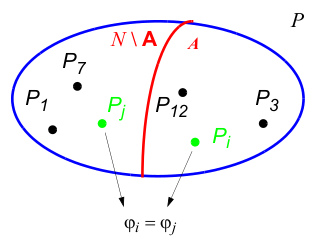
\includegraphics[scale=0.5]{Images/rice.png}
\end{center}

On utilise le plus souvent le théorème de Rice en ayant recourt à sa contraposée:

\begin{mytheo}[Rice (contraposée)]
	Si $\forall  i \in A$ et $\forall j \in \stcomp{A}$ on a $\varphi_i \neq \varphi_j$, alors $A$ est non-récursif ou $A = \emptyset$ ou $A = \N$.
\end{mytheo}

Dans de nombreux cas, on peut garantir $A \neq \emptyset$ et $A \neq \N$, ce qui permet de se servir de la contraposée pour démontrer qu'un ensemble est non-récursif sans utiliser la preuve par diagonalisation ou par réduction.

\begin{proof}
Nous avons que $\forall i \in A$ et $\forall j \in \stcomp{A}$, $\varphi_i \neq
\varphi_j$. Supposons $A$ récursif, $A \neq \emptyset$ et $A\neq \N$.

Dans cette démonstration, nous allons utiliser la méthode de réduction.
Sous l'hypothèse que $A$ est récursif, on montre que \textbf{HALT} est récursif en construisant un programme qui décide \textbf{HALT}.  Cela amène alors à une contradiction, car on sait que \textbf{HALT} n'est pas récursif.  Ce qui implique donc que $A$ ne peut pas être récursif.

\begin{enumerate}
	\item Construisons le programme suivant $P_k$ :
		\begin{lstlisting}
while true do;
		\end{lstlisting}

			$P_k$ ne s'arrête jamais, il vaut donc en permanence \textit{bottom} : $\forall x \ \varphi_k(x) = \bot$.

	\item $\stcomp{A}\neq \emptyset$ car $A \neq \N$,
	supposons $k\in \stcomp{A}$ (hypothèse sans importance, car montrer que
	$A$ ou $\stcomp{A}$ est non récursif revient au même, car $A$ non
	récursif $ \Leftrightarrow $ $\stcomp{A}$ non récursif).
	\item $A\neq \emptyset$ par hypothèse.  Prenons un élément quelconque $m$ de cet ensemble  ($m\in A$)
	\item Par hypothèse  $\forall i \in A, \forall j \in \stcomp{A}$ $\varphi_i\neq \varphi_j$.  Donc
		$\varphi_m \neq \varphi_k$.
	\item Pour $n$ et $x$ fixé, analysons le programme $P(z)$ suivant.
		$P(z) \equiv $
		\begin{lstlisting}
P_n(x);
P_m(z);
		\end{lstlisting}

			Ce programme a un numéro $d$.  Quelle est la fonction $\varphi_d(z)$ calculée par $P(z)$ ? Il n'y a que deux possibilités.
			\begin{itemize}
				\item Si $P_n(x)$ ne se termine pas, alors le programme $P(z)$ ne se termine pour aucune valeur de $z$. On a donc $\varphi_d =\varphi_k$.
				\item Si $P_n(x)$ se termine, alors le programme $P(z)$ calcule la même fonction que $P_m(z)$. On a donc $\varphi_d =\varphi_m$.
			\end{itemize}

Pour déterminer si $\varphi_d =\varphi_k$ ou  $\varphi_d =\varphi_m$, il suffit de tester si $d \in A$.   Par hypothèse  $\forall i \in A, \forall j \in \stcomp{A}$ $\varphi_i \neq \varphi_j$.  Nous avons aussi $k\in \stcomp{A}$ et $m\in A$.
			\begin{itemize}
            \item Si $d \in A$, alors  $\varphi_d \neq \varphi_k$, donc $\varphi_d =\varphi_m$.
            \item Si $d \in \stcomp{A}$, alors  $\varphi_d \neq \varphi_m$, donc $\varphi_d =\varphi_k$.
			\end{itemize}
En résumé : si $d \in A$ alors l'exécution de $P_n(x)$ se termine, sinon l'exécution de $P_n(x)$ ne se termine pas.

		On peut alors écrire le programme suivant qui décide \textbf{HALT}.
		 $halt(n,x) \equiv $
		\begin{lstlisting}
construire un programme P(z)= P_n(x); P_m(z);
d <- numero de P(z);
if d in A then print(1);
else print(0);
		\end{lstlisting}


	\item Contradiction, car \textbf{HALT} n'est pas récursif.
	\item Conclusion: $A$ n'est pas récursif.
\end{enumerate}
\end{proof}

\subsection{Analyse}

\paragraph{} En tenant compte du théorème de Rice, il est maintenant possible de différencier quelles propriétés d'un programme sont déterminables par un algorithme et lesquelles ne le sont pas.

\begin{itemize}
	\item \textbf{Si} la propriété est vérifiée par certains programmes, mais pas tous,
		et qu'elle est décidable, \textbf{alors} il existe deux programmes calculant la
		même fonction, mais l'un vérifie la propriété, et l'autre pas.

	\item \textbf{Si} une propriété de la fonction calculée par un programme est vérifiée par un programme, mais pas tous,
		\textbf{alors} cette propriété ne peut-être décidée par un algorithme.

	\item \textbf{S}'il existe un algorithme permettant de déterminer si un
		programme quelconque calcule une fonction ayant cette propriété,
		\textbf{alors} toutes les fonctions calculables ont cette propriété ou
		aucune fonction calculable n'a cette propriété.

	\item Aucune question relative aux programmes, vu sous l'angle de la
		fonction qu'ils calculent, ne peut être décidée par
		l'application d'un algorithme.

	\item Les propriétés intéressantes d'un programme concernant la
		fonction qu'il calcule, non pas sa forme (syntaxe), sont non calculables.

	\item La plupart des problèmes intéressants au sujet des programmes sont non calculables
\end{itemize}

\subsection{Exemples}

\paragraph{}Pour cela, considérons $A$ comme étant l'ensemble des programmes qui
respectent une propriété. Voici quelques exemples et applications du théorème de Rice.

\begin{description}
	\item[$A_1 =$] $\{i| \varphi_i \; \text{est totale}\}$ \\
	 				$P_i$ s'arrête toujours.
	\item[$A_2 =$] $\{i| \varphi_i = f\}$ avec f fixée \\
					$P_i$ calcule la fonction f.
	\item[$A_3 =$] $\{i| a \in \dom(\varphi_i)\}$ avec a fixé \\
					$P_i(a)$ se termine.
	\item[$A_4 =$] $\{i| \varphi_i(X) = \perp \text{pour tout X}\}$ \\
					$P_i$ calcule la fonction partielle vide.
	\item[$A_5 =$] $\{i| a \in \image(\varphi_i)\}$ avec a fixé \\
					$P_i$ donne au moins une fois le résultat a.
	\item[$A_6 =$] $\{i| \image(\varphi_i) = \N\}$ \\
					$P_i$ donne tous les résultats possibles.
	\item[$A_7 =$] $\{i| \varphi_i \text{est une fonction injective}\}$ \\
					$P_i$ calcule une fonction injective.
\end{description}

L'ensemble $A_1, \cdots, A_7$ est non récursif, par la contraposée du théorème de Rice. L'ensemble inverse $\stcomp{A_1}, \cdots, \stcomp{A_7}$ n'est par conséquent par récursif non plus.

% subsection th_or_me_de_rice (end)

\section{Théorème de la paramétrisation}
\label{sec:th_or_me_de_la_param_trisation}

\subsection{Transformation de programmes}
\label{sub:transformation_de_programmes}
\begin{mydef}[Transformateur de programme]
	On peut voir une fonction f: $\N \rightarrow \N$ comme une fonction qui prend
	le numéro d'un programme et qui retourne le numéro d'un autre programme f: $P
	\rightarrow P$. Donc on peut voir $P_k$, le programme qui calcule f comme un
	transformateur de programme. En effet, $P_k$ prend un programme en entrée et
	retourne un programme qui peut être différent.
\end{mydef}

\begin{mytheo}[S-m-n]
	\label{S-m-n}Pour tout $m,n \geq 0$, \\
	il existe une fonction totale calculable $S^m_n : \N^{m+1} \rightarrow
	\N$ \\
	telle que pour tout $k$ ($\varphi_k$ est calculable),
	$$ \varphi^{(n+m)}_k(x_1,...,x_n,x_{n+1},...,x_{n+m}) =
	\varphi^{(n)}_{S^m_n(k,x_{n+1}, ...,x_{n+m})} (x_1,...,x_n)$$
\end{mytheo}

\begin{proof}
	Pour prouver que $S^m_n$ est totale calculable, on va montrer comment construire un programme qui
	calcule  $S^m_n(k,x_{n+1}, ...,x_{n+m})$.\\
	Tout d'abord, comme $\varphi_k$ est calculable, il existe un programme
	$P_k(x_1,x_2,...,x_{n+m})$.\\
	On peut donc construire un programme $Q(x_1,...,x_n)$ qui calcule
	$P_k(x_1,x_2,...,x_{n+m})$.\\
	$x_1,...,x_n$ restent des arguments du programme,
	tandis que $x_{n+1},...,x_{n+m}$ deviennent des valeurs fixées.\\
	Notre programme qui calcule $S^m_n(k,x_{n+1}, ...,x_{n+m})$ n'a plus
	qu'à retourner le numéro du programme $Q$.\\
       	En résumé, $S^m_n(k,x_{n+1},
	...,x_{n+m}) \equiv$
	\begin{lstlisting}
construire Q(x1,x2,...,xn) = P_k(x1,x2,...xn,...,xn+m);
d <- numero du programme Q;
print(d);
	\end{lstlisting}
\end{proof}

\begin{mytheo}[S]
	C'est la propriété S-m-n affaiblie.
	\[ \forall \ k \ \exists \ S \ \text{(totale calculable)} : \varphi_k(x,y)=\varphi_{S(y)}(x)\]
	% Lena : j'ai plutôt ceci (c'est équivalent)
	% $$ \forall \text{ programme } P, \exists S \text{ totale calculable }:
	% P(x,y) \equiv \left[S(y) \right](x) $$
\end{mytheo}

\begin{proof}
Par le théorème \ref{S-m-n} (S-m-n),
	\[ \exists \ S \text{ (totale calculable) } \forall \ k : \varphi_k(x,y)=\varphi_{S(k,y)}(x)\]
	\[\Rightarrow \forall \ k \ \exists \ S \ \text{ (totale calculable) } : \varphi_k(x,y)=\varphi_{S(k,y)}(x)\]
    Pour un $k$ donné, on note $S_k(y)=S(k,y)$. $S_k$ est calculable puisque $S$ l'est. On a bien $\varphi_k(x,y) = \varphi_{S_k(y)}(x)$.
\end{proof}

\begin{myrem}
	On peut voir le théorème \ref{S-m-n}, S-m-n, comme : \\
	Étant donné $m,n \geq 0$, il existe un transformateur de programme, $S^m_n$, qui recevant comme
	données un programme $P_k$ à $n+m$ arguments et $m$ valeurs $v_1,...,v_m$
	fournit comme résultat un programme $P$ à $n$ arguments tel que
	$P(x_1,...,x_n)$ calcule la même fonction que
	$P_k(x_1,...,x_n,,v_1,...,v_m)$ (ce programme effectue une projection)
\end{myrem}

\begin{myrem}
	On peut donc voir la transformation de programmes $S^m_n$ comme un
	programme qui particularise un autre programme à $m+n$ argument en rendant
	constant les m derniers paramètres.
\end{myrem}

\section{Théorème du point fixe}
\label{sec:th_or_me_du_point_fixe}
\begin{mytheo}[Point fixe]
	\label{point-fixe}
    Soient $n \geq 0$ et $f$ fonction totale
	calculable, il existe $k$ tel que $\varphi^{(n)}_k = \varphi^{(n)}_{f(k)}$.
\end{mytheo}

\begin{myrem}
	Le théorème \ref{point-fixe} n'est pas très intuitif. Mais on peut le
	voir comme : quel que soit un transformateur de programme T qui calcule f (n'importe quelle fonction totale calculable peut être vue comme un transformateur	de programme),
	il existe deux programmes $P_k$ et $P_j$ tels que
	\begin{itemize}
		\item $P_j$ est la transformation de $P_k$ via T,
		\item $P_k$ et $P_j$ calcule la \textbf{même} fonction.
	\end{itemize}
\end{myrem}

\begin{proof}
Pour commencer la démonstration, on va sortir 3 ``lapins'' d'un chapeau (analogie aux tours de magie) :
\begin{description}
	%\item $h(u,v) =$
	%	\begin{tabular}{c}
	%		$\varphi_{\varphi_{u(u)}}(v)$ si $\varphi(u)\neq \perp$\\
	%		$\perp$ sinon
	%	\end{tabular}\\

	\item[$1^{er}$ lapin:] Soit $ h(u,v) = \left\{
	\begin{array}{l l}
		\varphi_{\varphi_{u}(u)}(v) & \quad \text{si }\varphi_u(u)\neq \bot,\\
    	\bot & \quad \text{sinon}.
	\end{array} \right.$

		$h$ est calculable
		\begin{myrem}
			on peut créer un programme qui calcule $h$ :
            \begin{algorithmic}
              \STATE Input: $u,v$
              \STATE $a = P_z(u,u)$
              \STATE $P_z(a,v)$
            \end{algorithmic}
            où $\varphi_z = \theta$ est la fonction universelle.
		\end{myrem}

	\item[$2^{eme}$ lapin:] $h(u,v)=\varphi_{S(u)}(v)$\\
	Ceci est une application de la propriété S (propriété S-m-n affaiblie), avec $S$ totale calculable.

	\item[$3^{eme}$ lapin:] Soit $g(u)=f(S(u))$\\
	 $g$ est totale calculable car $S$ et $f$ le sont ($f$
		est la fonction donnée dans le théorème).
		\[ \exists k' \text{ tel que } \varphi_{k'}(u) =g(u)=f(S(u)) \]
\end{description}
On a que $k'$ est une constante et par le lapin 2 :
\[h(k',v) = \varphi_{S(k')}(v)\]
Par le lapin 1 et car $g=\varphi_{k'}$ est une fonction totale calculable, on a :
\[h(k',v) = \varphi_{\varphi_{k'}(k')}(v)\]
Par le lapin 3, on a que $\varphi_{k'}(u) = g(u)=f(S(u))$ donc :
\[h(k',v) = \varphi_{f(S(k'))}(v)\]
Par le lapin 2, on a:
\[ \varphi_{S(k')}(v) =\varphi_{f(S(k'))}(v) \]
Si on pose que $S(k')=k$ on a bien
\[ \varphi_{k}(v) = \varphi_{f(k)}(v) \]
Ce qui conclut notre démonstration.
		\begin{myrem}
          La fonction $S(k')$ pourrait produire le programme suivant :
          \begin{algorithmic}
            \STATE Input: $v$
            \STATE $a = P_z(k',k')$
            \STATE $P_z(a,v)$
          \end{algorithmic}
          On remarque que comme $S$ et $f$ sont totales,
          $g$ l'est aussi donc $P_z(k',k')$ se terminera toujours et donne pour résultat $f(S(k'))$ (lapin 3).

          Que se passe-t-il quand on exécute le programme généré par $S(k')$ sur une donnée $v$ quelconque ?
          La seconde instruction se termine et on obtient $a = f(S(k'))$.
          Ensuite on exécute le programme $P_z(a,v) = P_a(v)$ qui fournit le résultat final. \\
          Exécuter le programme généré par $S(k')$ sur une donnée $v$ revient donc à exécuter le programme $f(S(k'))$ sur cette donnée $v$.
          On a donc
          \[ \varphi_{S(k')} = \varphi_{f(S(k'))}. \]
          Le programme $S(k')$ est bien un point fixe de $f$.
		\end{myrem}
\end{proof}

\begin{myrem}[Conséquences Point fixe]

Grâce à ce théorème qui se base sur l'unique propriété de S, nous pouvons démontrer plein de choses comme:
\begin{itemize}
   \item HALT non-calculable
   \item Le théorème de Rice
   \item Le théorème de Hoare-Allison via la démonstration de HALT non-calculable
\end{itemize}
Le théorème du point fixe c'est la base de la calculabilité. Il fixe toutes les limites de la calculabilité.
 
\end{myrem}

\begin{myrem}[Démonstration du théorème de Rice grâce au point fixe]
  À l'aide du point fixe, on peut démontrer plus simplement le théorème de Rice:

\begin{center}
Si $A$ est récursif et $A \neq \emptyset \neq \bar{A}$, alors il existe $i \in A$ et $j \in \bar{A}$ tel que $\varphi_i = \varphi_j$.
\end{center}

  \begin{proof}
    Soit un ensemble $A$ tel que $A \neq \emptyset$ et $\bar{A} \neq \N$.  Il suffit de montrer que si
    $\forall i \in A, \forall j \in \bar{A} : \varphi_i \neq \varphi_j$  (1) alors A est non récursif. \\
    En supposant A récursif, on arrive à une contradiction.  En effet,
    soit $n \in A$ et $m \in \bar{A}$, définissons la fonction
    \[
      f(x) =
      \begin{cases}
        m & \text{si }x \in A,\\
        n & \text{si }x \in \bar{A}.
      \end{cases}
    \]
    Comme $A$ est récursif, la fonction $f$ est total calculable.
    Dès lors, par le théorème du point fixe, il existe $k$ tel que
    \[ \varphi_{f(k)} = \varphi_k \]
    La valeur $k$ est-elle dans $A$ ou dans $\bar{A}$ ?
    \begin{itemize}
      \item Si $k \in A$, alors $f(k)=m$.  On a donc $\varphi_m = \varphi_k$, ce qui est contradictoire avec (1) car
       $m \in \bar{A}$.
      \item Si $k \in \bar{A}$, alors $f(k)=n$.  On a donc $\varphi_n = \varphi_k$, ce qui est contradictoire avec (1) car
        $n \in A$.
    \end{itemize}
  \end{proof}
\end{myrem}

\begin{myrem}[Démonstration de $K$ grâce au point fixe]
	On peut démontrer que $K$ n'est pas récursif.

    \begin{proof}
	Soit $n$ un programme qui ne s'arrête jamais, et $m$ un programme qui calcule la fonction identité:
		\begin{itemize}
		\item $\varphi_n(x) = \bot \quad \forall \ x$
		\item $\varphi_m(x) = x \quad \forall  \ x$
	\end{itemize}
	Posons maintenant la  fonction suivante :
	\begin{itemize}

		\item $ f(x) = \left\{
		\begin{array}{l l}
			n & \quad \text{si $x\in$ K}\\
    		m & \quad \text{si $x\notin$ K}
		\end{array} \right.$
	\end{itemize}

    On montre que par construction pour tout $k$, $\varphi_{f(k)} \neq \varphi_k$.
    \begin{itemize}
      \item Si $k \in K$, $\varphi_k(k) \neq \bot$, $f(k) = n$ et
        $\varphi_{f(k)}(k) = \varphi_n(k) = \bot \neq \varphi_k(k)$ donc $\varphi_{f(k)} \neq \varphi_k$.
      \item Si $k \notin K$, $\varphi_k(k) = \bot$, $f(k) = m$ et
        $\varphi_{f(k)}(k) = \varphi_m(k) \neq \bot = \varphi_k(k)$ donc $\varphi_{f(k)} \neq \varphi_k$.
    \end{itemize}
    Si $K$ est récursif, alors $f$ est total calculable.
	Par le théorème du point fixe, il existe $k$ tel que $\varphi_k = \varphi_{f(k)}$.
    Ce qui est contradictoire.

    $K$ n'est donc pas récursif.
  \end{proof}

\end{myrem}

\section{Autres problèmes non calculables}
\label{sec:autres_probl_mes_non_calculable}

\begin{mydef}[Problème de correspondance de Post] Soit deux listes U et V
	de mots non vides sur un alphabet $\Sigma$ :
	\begin{itemize}
		\item U = ${u_1,u_2,...,u_k}$
		\item V = ${v_1,v_2,...,v_k}$
	\end{itemize}
	Le problème consiste à décider s’il existe une suite d'entiers
	$i_1,i_2,..,i_n$ telle que les mots $u_{i_1},u_{i_2},...,u_{i_n}$ et
	$v_{i_1},v_{i_2},...,v_{i_n}$ soient \textbf{identiques}. \\
	Pour démontrer l'indécidabilité de ce problème, Post à introduit un
	nouveau modèle, la machine de Post qui ressemble à une machine de Turing.
\end{mydef}

% en français, on écrit ``diophantiennes'', en anglais ``diophantines''
\begin{mydef}[Problème des équations diophantiennes]
  Décider si une équation
  polynomiale de degré supérieur ou égal à 4 possède une solution entière.
\end{mydef}
C'est le 10\ieme{} problème de Hilbert, résolu en 1970 par Matiyasevich;
voir \cite{davis1973hilbert} pour une description de la solution et des remarques historiques.
Ce résultat implique, en particulier, qu'il n'existe pas d'algorithme pour résoudre
la programmation quadratique entière; voir \cite{jeroslow1973there}.
Un bon aperçu des questions de non décidabilité pour les équation polynomiale est \cite{koenigsmann2014undecidability}.

Il n'existe pas d'algorithme résolvant ces problèmes. Il existe beaucoup
d'autres problèmes non calculables. Il y a d'autres exemples sur les grammaires dans le cours.
% subsection autres_probl_mes_non_calculable (end)

\section{Nombres calculables}
\label{sec:nombres_calculables}

\begin{mydef}[Nombre réel]
	Un nombre réel est défini comme la limite d'une suite (convergente) de
	nombres rationnels: $\lim_{n \rightarrow +\infty} |x-s(n)| = 0 $ ou $s$ est
	une fonction totale.
\end{mydef}

\begin{mydef}[Nombre réel calculable]
	Un nombre réel x est calculable s’il existe une fonction totale
	calculable $s$ tel que pour tout $n$  : $|x-s(n)| \leq 2^{-n}$.
\end{mydef}

\begin{myrem}
	Donc un nombre est calculable s'il existe un programme qui peut
	l'approximer aussi près que l'on veut. Par exemple $\pi$ et $e$ sont
	calculables
\end{myrem}

\begin{myprop}
	L'ensemble des nombres réels calculables est énumérable, car on peut énumérer les
	fonctions totales calculables.
\end{myprop}

\begin{myprop}
	Il existe des nombres réels non calculables.
\end{myprop}

\begin{myprop}
	Il existe des nombres réels non calculables qui peuvent être définis de
	manière finie.\footnote{Par exemple l'Oméga de Chaitin, qui est défini comme étant la probabilité qu’un programme auto-délimité, généré aléatoirement, finisse par s'arrêter.}
\end{myprop}

% subsection nombres_calculables (end)

\section{Conclusion}
[Conclusion très partielle...]\\
Le théorème S-m-n permet de démontrer le théorème du point fixe.
Le théorème du point fixe est un résultat central de la calculabilité. Il
implique le théorème de Rice, la non-récursivité de K et la non-calculabilité
de la fonction halt.

% subsection conclusion (end)
% section r_sultats_fondamentaux (end)
